\documentclass[10pt]{beamer}\usepackage[]{graphicx}\usepackage[]{color}
% maxwidth is the original width if it is less than linewidth
% otherwise use linewidth (to make sure the graphics do not exceed the margin)
\makeatletter
\def\maxwidth{ %
  \ifdim\Gin@nat@width>\linewidth
    \linewidth
  \else
    \Gin@nat@width
  \fi
}
\makeatother

\definecolor{fgcolor}{rgb}{0.345, 0.345, 0.345}
\newcommand{\hlnum}[1]{\textcolor[rgb]{0.686,0.059,0.569}{#1}}%
\newcommand{\hlstr}[1]{\textcolor[rgb]{0.192,0.494,0.8}{#1}}%
\newcommand{\hlcom}[1]{\textcolor[rgb]{0.678,0.584,0.686}{\textit{#1}}}%
\newcommand{\hlopt}[1]{\textcolor[rgb]{0,0,0}{#1}}%
\newcommand{\hlstd}[1]{\textcolor[rgb]{0.345,0.345,0.345}{#1}}%
\newcommand{\hlkwa}[1]{\textcolor[rgb]{0.161,0.373,0.58}{\textbf{#1}}}%
\newcommand{\hlkwb}[1]{\textcolor[rgb]{0.69,0.353,0.396}{#1}}%
\newcommand{\hlkwc}[1]{\textcolor[rgb]{0.333,0.667,0.333}{#1}}%
\newcommand{\hlkwd}[1]{\textcolor[rgb]{0.737,0.353,0.396}{\textbf{#1}}}%
\let\hlipl\hlkwb

\usepackage{framed}
\makeatletter
\newenvironment{kframe}{%
 \def\at@end@of@kframe{}%
 \ifinner\ifhmode%
  \def\at@end@of@kframe{\end{minipage}}%
  \begin{minipage}{\columnwidth}%
 \fi\fi%
 \def\FrameCommand##1{\hskip\@totalleftmargin \hskip-\fboxsep
 \colorbox{shadecolor}{##1}\hskip-\fboxsep
     % There is no \\@totalrightmargin, so:
     \hskip-\linewidth \hskip-\@totalleftmargin \hskip\columnwidth}%
 \MakeFramed {\advance\hsize-\width
   \@totalleftmargin\z@ \linewidth\hsize
   \@setminipage}}%
 {\par\unskip\endMakeFramed%
 \at@end@of@kframe}
\makeatother

\definecolor{shadecolor}{rgb}{.97, .97, .97}
\definecolor{messagecolor}{rgb}{0, 0, 0}
\definecolor{warningcolor}{rgb}{1, 0, 1}
\definecolor{errorcolor}{rgb}{1, 0, 0}
\newenvironment{knitrout}{}{} % an empty environment to be redefined in TeX

\usepackage{alltt}


%\input{slides_header.tex}
\usepackage{graphicx}
\usepackage{hyperref, url}
\hypersetup{colorlinks,citecolor=myorange,filecolor=red,linkcolor=brown,urlcolor=blue}

\usepackage{longtable,booktabs}
\usepackage{amssymb,amsmath}
\usepackage{animate}
\usepackage{subfig}
\usepackage{tikz}
\usetikzlibrary{shapes.geometric, arrows,shapes.symbols,decorations.pathreplacing}
\tikzstyle{startstop} = [rectangle, rounded corners, minimum width=3cm, minimum height=1cm, draw=black, fill=pinkish,text width=3.5cm]
\tikzstyle{startstop2} = [rectangle, rounded corners, minimum width=3cm, minimum height=1cm, draw=black, fill=background,text width=4.5cm]
\tikzstyle{startstop3} = [rectangle, rounded corners, minimum width=3cm, minimum height=1cm, draw=black, fill=beige,text width=3.0cm]
\tikzstyle{startstop4} = [rectangle, rounded corners, minimum width=3cm, minimum height=1cm, draw=black, fill=pinkish,text width=4.5cm]
\tikzstyle{io} = [trapezium, trapezium left angle=70, trapezium right angle=110, minimum width=2cm, minimum height=1cm, text centered, draw=black, fill=blue!30,text width=1.5cm]
\tikzstyle{process} = [rectangle, minimum width=1cm, minimum height=1cm, text centered, draw=black, fill=orange!30,text width=2cm]
\tikzstyle{decision} = [diamond, minimum width=2cm, minimum height=1cm, text centered, draw=black, fill=green!30]
\tikzstyle{arrow} = [thick,->,>=stealth]
\tikzstyle{both} = [thick,<->,>=stealth, red]


% used for tree of stats tests in 001-introduction
\tikzstyle{startstopstats} = [rectangle, rounded corners, minimum width=2cm, minimum height=.5cm,text centered, draw=black, fill=red!30]
\tikzstyle{iostats} = [trapezium, trapezium left angle=70, trapezium right angle=110, minimum width=2cm, minimum height=.5cm, text centered, draw=black, fill=blue!30]
\tikzstyle{processstats} = [rectangle, minimum width=1.5cm, minimum height=.5cm, text centered, draw=black, fill=orange!30]
\tikzstyle{processbigstats} = [rectangle, minimum width=1.5cm, minimum height=.5cm, text centered, draw=black, fill=orange!30,text width=1.6cm]
\tikzstyle{decisionstats} = [rectangle, minimum width=1cm, minimum height=1cm, text centered, draw=black, fill=green!30,text width=1.6cm]
\tikzstyle{decisionbigstats} = [rectangle, minimum width=1cm, minimum height=1cm, text centered, draw=black, fill=yellow!30,text width=2cm]

\usepackage{pifont}% http://ctan.org/pkg/pifont
\newcommand{\cmark}{\ding{51}}%
\newcommand{\xmark}{\ding{55}}%

\usepackage{ulem} % for strikeout

\usepackage{xcolor}
\usepackage{color, colortbl}
\definecolor{lightgray}{RGB}{200,200,200}
\definecolor{palegray}{RGB}{221,221,221}
\definecolor{myblue}{RGB}{0,89,179}
\definecolor{myorange}{rgb}{0.776,0.357,0.157}
\definecolor{gray}{RGB}{110,110,110}
\definecolor{darkgray}{RGB}{100,100,100}
\definecolor{lightgray}{RGB}{200,200,200}
\definecolor{palegray}{RGB}{221,221,221}
\definecolor{turquoise}{RGB}{81,193,188}
\definecolor{tomato}{RGB}{255,136,136}
\definecolor{mandarina}{RGB}{229,169,25}
\definecolor{foreground}{RGB}{81,141,193}
\definecolor{background}{RGB}{246,244,240}
\definecolor{highlight}{RGB}{229,169,25}
\definecolor{lowlight}{RGB}{200,200,200}
\definecolor{beige}{RGB}{255,255,240}
\definecolor{pinkish}{RGB}{255,223,247}
\definecolor{darktangerine}{rgb}{1.0, 0.66, 0.07}
\definecolor{deepink}{RGB}{255,20,147}
%\usepackage{shadethm}
%\colorlet{shadecolor}{blue!15}
%\colorlet{shadecolor}{palegray}
%\setlength{\shadeboxrule}{.4pt}

%\newshadetheorem{thm}{Theorem}
%\newshadetheorem{defm}{Definition}
%\newshadetheorem{exm}{Exercise}
%\newshadetheorem{remarkm}{Remark}
%\definecolor{shadethmcolor}{HTML}{EDF8FF}
%\definecolor{shadethmcolor}{RGB}{221,221,221}
%\definecolor{shaderulecolor}{HTML}{45CFFF}
%\definecolor{shaderulecolor}{RGB}{0,89,179}
%\setlength{\shadeboxrule}{.4pt}



\usepackage{epsfig}

\newcommand{\code}[1]{\texttt{#1}}
\newcommand{\blue}[1]{\textcolor{blue}{#1}}
\newcommand{\red}[1]{\textcolor{red}{#1}}

\usepackage{comment}

\makeatletter

\def \iqsssectiontitleheader {}

\newcommand{\iqsssectiontitle}[1]{
	\def \iqsssectiontitleheader{#1}
}

\@ifundefined{insertmainframenumber}
{%
	% \insertmainframenumber not defined
	\newcommand{\insertmainframenumber}{\inserttotalframenumber}
}
{%
	% \insertmainframenumber already defined
}%


\AtBeginSection[]{
	\title{\insertsectionhead}
	{
		%\definecolor{white}{RGB}{140,193,250}
		%\definecolor{white}{RGB}{200,200,200}
		%\definecolor{white}{RGB}{242,244,247}
		\definecolor{white}{RGB}{0,89,179}
		%\definecolor{iqss@orange}{rgb}{1,1,1}
		\ifnum \insertmainframenumber > \insertframenumber
		%\setbeamercolor{background canvas}{bg=myblue}
		%\setbeamercolor{normal text}{fg=black,bg=white}
		%\setbeamercolor{frametitle}{fg=red}
		%\setbeamercolor{section in toc}{fg=myblue, bg=white}
		%\setbeamercolor{subsection in toc}{fg=myblue, bg=white}
		\frame{
			\frametitle{\iqsssectiontitleheader}
			\tableofcontents[currentsection]
		}
		\else
		\frame{
			\frametitle{Backup Slides}
			\tableofcontents[sectionstyle=shaded/shaded,subsectionstyle=shaded/shaded/shaded]
		}
		\fi
	}
}
\makeatother
%\graphicspath{{/home/sahir/git_repositories/EPIB607/resources/assets/slides/figure/}}


\usepackage{fontspec}
%\setsansfont{Fira Sans}
%\setmonofont{Fira Mono}
%\setsansfont[ItalicFont={Fira Sans Light Italic},BoldFont={Fira Sans},BoldItalicFont={Fira Sans Italic}]{Fira Sans Light}
%\setmonofont[BoldFont={Fira Mono Medium}]{Fira Mono}

\def\installpath{/usr/local/share/texmf/fonts/opentype/libertinus/}
\setmainfont{LibertinusSerif}[
UprightFont    = *-Regular,
BoldFont       = *-Bold,
ItalicFont     = *-Italic,
BoldItalicFont = *-BoldItalic,
Ligatures      = TeX,
Extension      = .otf,
Path           = \installpath/
]

\setsansfont{LibertinusSerif}[
UprightFont    = *-Regular,
BoldFont       = *-Bold,
ItalicFont     = *-Italic,
BoldItalicFont = *-BoldItalic,
Ligatures      = TeX,
Extension      = .otf,
Path           = \installpath/
]


%\setmonofont{LibertinusSerif}[
%UprightFont    = *-Regular,
%BoldFont       = *-Bold,
%ItalicFont     = *-Italic,
%BoldItalicFont = *-BoldItalic,
%Ligatures      = TeX,
%Extension      = .otf,
%Path           = \installpath/
%]






\newcommand\Wider[2][3em]{%
	\makebox[\linewidth][c]{%
		\begin{minipage}{\dimexpr\textwidth+#1\relax}
			\raggedright#2
		\end{minipage}%
	}%
}


\newcommand {\framedgraphic}[1] {
	\begin{figure}
		\centering
		\includegraphics[width=\textwidth,height=0.9\textheight,keepaspectratio]{#1}
	\end{figure}
}


\newcommand {\framedgraphiccaption}[2] {
	\begin{figure}
		\centering
		\includegraphics[width=\textwidth,height=0.8\textheight,keepaspectratio]{#1}
		\caption{#2}
	\end{figure}
}




\setbeamercolor{itemize item}{fg=myblue}
\setbeamercolor{itemize subitem}{fg=myorange}
%\setbeamertemplate{itemize item}[square]
\setbeamertemplate{itemize item}[circle]
\setbeamertemplate{itemize subitem}[triangle]
\setbeamertemplate{blocks}[rounded][shadow=true]
\setbeamercolor{block body alerted}{bg=alerted text.fg!10}
\setbeamercolor{block title alerted}{bg=alerted text.fg!20}
\setbeamercolor{block body}{bg=structure!10}
\setbeamercolor{block title}{bg=structure!20}
\setbeamercolor{block body example}{bg=green!10}
\setbeamercolor{block title example}{bg=green!20}


\makeatletter
\newenvironment<>{proofs}[1][\proofname]{%
	\par
	\def\insertproofname{#1\@addpunct{.}}%
	\usebeamertemplate{proof begin}#2}
{\usebeamertemplate{proof end}}
\newenvironment<>{proofc}{%
	\setbeamertemplate{proof begin}{\begin{block}{}}
		\par
		\usebeamertemplate{proof begin}}
	{\usebeamertemplate{proof end}}
	\newenvironment<>{proofe}{%
		\par
		\pushQED{\qed}
		\setbeamertemplate{proof begin}{\begin{block}{}}
			\usebeamertemplate{proof begin}}
		{\popQED\usebeamertemplate{proof end}}
\makeatother


\makeatletter
\newenvironment<>{exams}[1][\proofname]{%
	\par
	\def\insertproofname{#1\@addpunct{.}}%
	\usebeamertemplate{example begin}#2}
{\usebeamertemplate{example end}}
\newenvironment<>{examc}{%
	\setbeamertemplate{exam begin}{\begin{block}{}}
		\par
		\usebeamertemplate{exam begin}}
	{\usebeamertemplate{exam end}}
	\newenvironment<>{exame}{%
		\par
		\pushQED{\qed}
		\setbeamertemplate{exam begin}{\begin{block}{}}
			\usebeamertemplate{exam begin}}
		{\popQED\usebeamertemplate{exam end}}
		\makeatother

%\definecolor{mycolor}{HTML}{F7F8E0}
%\declaretheorem[shaded={bgcolor=mandarina}]{theo}
%\declaretheorem[shaded={bgcolor=mycolor}]{propo}
%\declaretheorem[shaded={bgcolor=green!80!black!30}]{remark}

%\setbeamertemplate{navigation symbols}{\usebeamercolor[fg]{title in head/foot}\usebeamerfont{title in head/foot}\insertframenumber}


%\setbeamertemplate{footline}{}

\beamertemplatenavigationsymbolsempty % toggle off if you want navigation symbols at the bottom

\setbeamertemplate{footline}
{ \usebeamercolor[fg]{page number in head/foot}%
	\usebeamerfont{page number in head/foot}%
	\hspace{1em}\insertsectionhead%
	\hfill%
	\insertframenumber\,/\,\hyperlinkappendixstart{\insertmainframenumber}
	\ifnum \thepage = \insertframeendpage{\small .}\else{\phantom{\small .}}\fi
	\hspace{1em}
	\vskip2pt%
}

%\newtheorem{proposition}[theorem]{Proposition}
%\newtheorem{exercise}[theorem]{Exercise}
%\newtheorem{remark}[theorem]{Remark}


\usepackage{amsthm}
\usepackage{thmtools}

\setbeamertemplate{theorems}[ams style] 
%\setbeamertemplate{theorems}[numbered] 
%\setbeamertemplate{corollary}[numbered] 
\newtheorem{proposition}{Proposition}
\newtheorem{exercise}{Exercise}
\newtheorem{remark}{Remark}
\newtheorem{exam}{Example}
%\newtheorem{proof}{Proof}
%\newtheorem{corollaries}[theorem]{Corollary}
\newcommand*{\theorembreak}{\usebeamertemplate{theorem end}\framebreak\usebeamertemplate{theorem begin}}



\setlength{\emergencystretch}{3em} % prevent overfull lines
\providecommand{\tightlist}{%
	\setlength{\itemsep}{0pt}\setlength{\parskip}{0pt}}

\newcommand\AddButton{%
	\setbeamertemplate{background canvas}{%
		\begin{tikzpicture}[remember picture,overlay]
		\node[anchor=west] at ([yshift=5pt,xshift=0.1em]current page.south west)
		{\hyperlink{toc}{\beamergotobutton{back to TOC}}};
		\end{tikzpicture}%
	}%
}


\titlegraphic{\hfill
\includegraphics[height=1cm]{/home/sahir/git_repositories/EPIB607/slides/mcgill_logo.png}}




\graphicspath{{/home/sahir/git_repositories/EPIB607/slides/figure/}}

%\let\oldShaded\Shaded
%\let\endoldShaded\endShaded
%\renewenvironment{Shaded}{\footnotesize\oldShaded}{\endoldShaded}

\newcommand{\Var}{\operatorname{Var}}
\newcommand{\Expec}{\operatorname{E}}
\newcommand{\Prob}{\operatorname{P}}
\IfFileExists{upquote.sty}{\usepackage{upquote}}{}
\begin{document}
	
	

%\title{Introduction to Regression Trees}
%\author{Sahir Bhatnagar \inst{1}}
%\author[shortname]{Sahir Rai Bhatnagar, PhD Candidate (Biostatistics) }
%\institute[shortinst]{Department of Epidemiology, Biostatistics and Occupational Health}

	\title{011 - Normal Curves}
\author{EPIB 607}
\institute{
	Sahir Rai Bhatnagar\\
	Department of Epidemiology, Biostatistics, and Occupational Health\\
	McGill University\\
	
	\vspace{0.1 in}
	
	\texttt{sahir.bhatnagar@mcgill.ca}\\
	%\texttt{\url{https://sahirbhatnagar.com/EPIB607/}}
}

\date{slides compiled on \today}

\maketitle

\section{Normal Curves and Calculations}


\frame{\frametitle{The Normal (Gaussian) distribution} What is
	it?
	\begin{itemize}
		\item A distribution that describes continuous (numerical) data
		\item Can also be used to approximate discrete data distributions
		\item Range is (technically) infinite, though the probability of seeing
		very large or very small values is extremely tiny
		\item Fully described by only two parameters, the mean and variance
		($\mu$ and $\sigma^2$)
		\item \textcolor{red}{NOTE:} \texttt{R} use the short-hand: $X \sim
		\mathcal{N}(\mu,\sigma)$, denoting the normal distribution as a
		function of the mean and \textit{standard deviation}. This is not
		standard; many texts instead write $X \sim
		\mathcal{N}(\mu,\sigma^2)$. Be careful of this!
	\end{itemize}
} \frame{\frametitle{The Normal (Gaussian) distribution} Carl Gauss
	was a German mathematician who developed a number of important
	advances in statistics such as the method of least squares.
	\begin{figure}
		\begin{center}
			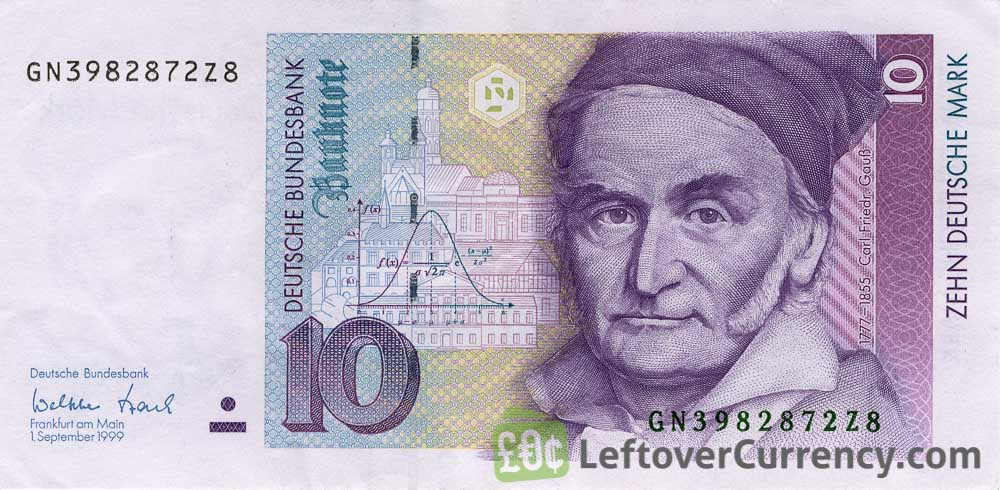
\includegraphics[scale=0.2]{gauss.jpg}
		\end{center}
		\caption{The Deutsche Bundesbank issued Deutsche Mark banknotes in 15 different denominations, including this 10 Deutsche Marks banknote featuring Carl Friedrich Gauss.}
	\end{figure}
} 

\frame{\frametitle{The Normal distribution} Where do Normal data
	come from?
	\begin{itemize}
		\item Natural processes
		\begin{itemize}
			\item Blood pressure
			\item Height
			\item Weight
			\item[]
		\end{itemize} \pause
		\item ``Man-made'' (or derived)
		\begin{itemize}
			\item Binomial (proportion) and Poisson (count) data are
			approximately Normal under certain conditions
			\item Sums and means of random variables (Central Limit Theorem)
			\item Data can sometimes be made to look Normal via transformations
			(squares, logs, etc)
		\end{itemize}
	\end{itemize}
} 

\frame{\frametitle{The Normal distribution} For Normal data, we
	can use \sout{the Gaussian tables} \texttt{R} to answer the questions:
	\begin{itemize}
		\item What is the probability that a single observation $X$ is
		\begin{itemize}
			\item greater than $X^*$?
			\item less than $X^*$?
			\item between $X^*_L$ and $X^*_U$?
		\end{itemize}
		\item That is, we can find out information about the percent
		distribution of $X$ as a function of thresholds $X^*$, or $X^*_L$
		and $X^*_U$.
		\item[] \pause
		\item We can also use \sout{the Normal tables} \texttt{R} to find out information about
		thresholds $X^*$ that will contain particular percentages of
		the data. I.e., we can find what threshold values will
		\begin{itemize}
			\item Exclude the lower $\omega^*$\% of a population
			\item Exclude the upper $\omega^*$\% of a population
			\item Contain the middle $\omega^*$\% of a population
		\end{itemize}
	\end{itemize}
}

\frame{\frametitle{The Normal distribution} We can use \sout{the
		Gaussian tables} \texttt{R} to answer these questions \textbf{no matter
		what the values
		of} $\mu$ and $\sigma^2$. \\ \ \\
	That is, the \% of the Normal distribution falling between $X^*_L =
	\mu - m_1\sigma$ and $X^*_U = \mu + m_2\sigma$ where
	$m_1, m_2$ are any multiples \textbf{remains the same} for any $\mu$ and $\sigma$. \\ \ \\
	How so?? \pause
	\begin{center}
		Because we can \textbf{standardize} any $X \sim
		\mathcal{N}(\mu,\sigma)$ to find $Z \sim \mathcal{N}(0,1)$
\end{center} }

\frame{\frametitle{The Normal distribution} An illustration
	using IQ scores, which we presume have a $\mathcal{N}(100,13)$
	distribution of scores. \\ \ \\
	
	\textcolor{blue}{Q1:} What percentage of scores are
	\textbf{above}
	130? \\
	Two steps:
	\begin{enumerate}
		\item Change of location from $\mu_X=100$ to $\mu_Z=0$
		\item Change of scale from $\sigma_X=13$ to $\sigma_Z=1$
		\item[]
	\end{enumerate}
	Together, this gives us \[Z = \frac{X-\mu_X}{\sigma_X} =
	\frac{130-100}{13} = 2.31\] }

\begin{frame}[fragile]{The Normal distribution}
	
	\vspace*{-.01in}
	
	\small{The position of $X$=130 in a $\mathcal{N}(100,13)$ distribution is the same as
		the place of $Z=2.31$ on the $\mathcal{N}(0,1)$, which we call the \textbf{standardized} Normal distribution (or	$Z$-distribution).}
	
	%\begin{figure}
	%		\begin{center}
	%			\epsfig{figure=Part1Figs/TwoNormals-equalProb.eps,width=4.4in,height=2.5in}
	%		\end{center}
	%	\end{figure}
	
\begin{knitrout}\tiny
\definecolor{shadecolor}{rgb}{0.969, 0.969, 0.969}\color{fgcolor}

{\centering 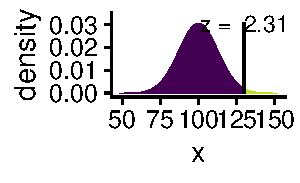
\includegraphics[width=0.55\linewidth]{figure/probs-1} 

}




{\centering 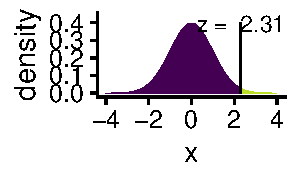
\includegraphics[width=0.55\linewidth]{figure/probs-2} 

}


\end{knitrout}
	
\end{frame} 

\frame{\frametitle{The Normal distribution} How are the
	values
	in the Normal tables found?\\ \ \\
	Normal density:
	\[f(x|\mu,\sigma) = \frac{1}{\sqrt{2\pi}\sigma}\exp\frac{-(x-\mu)^2}{2\sigma^2}\]
	
	\vspace{.5cm} Probabilities found by integration (area under the
	Normal curve): \[ P(a \le x \le b) =
	\int_a^b\frac{1}{\sqrt{2\pi}\sigma}\exp\frac{-(x-\mu)^2}{2\sigma^2}dx\]
}


\frame{\frametitle{The Normal distribution} (The percent above
	$X=130$) = (\% above $Z=2.31$) =1.04\%\\ \ \\
	
	How do we know this? We look at the lower tail probability of
	2.31 [i.e., the \% below 2.31], and then subtract it from 1:
	\begin{enumerate}
		\item $P(X < 130) = P(Z < 2.31) = 0.9896$
		\item $P(X > 130) = 1 - P(X < 130) = 0.0104$
		\item[]
	\end{enumerate}
	So 130 is the 98.96$^{th}$ percentile of a $\mathcal{N}$(100,13)
	distribution. }


\begin{frame}{Reminder about percentiles and quantiles}
	
	\begin{itemize}
		\item \textbf{Quantile}
		\begin{itemize}
			\item Any set of data, arranged in ascending or descending order, can be divided into various parts, also known as partitions or subsets, regulated by quantiles. 
			\item Quantile is a generic term for those values that divide the set into partitions of size $n$, so that each part represents $1/n$ of the set. 
			\item Quantiles are not the partition itself. They are the numbers that define the partition. 
			\item You can think of them as a sort of numeric boundary.
		\end{itemize}
	\end{itemize}
	\pause 
	
	\begin{itemize}
		\item \textbf{Percentile}
		\begin{itemize}
			\item Percentiles are quite similar to quantiles: they split your set, but only into two partitions. 
			\item For a generic $k$th percentile, the lower partition contains k\% of the data, and the upper partition contains the rest of the data, which amounts to 100 - k \%, because the total amount of data is 100\%. 
			\item Of course k can be any number between 0 and 100.
		\end{itemize}
	\end{itemize}
	
\end{frame}



\begin{frame}{More about percentiles and quantiles}
	\begin{itemize}
		\item In class, we will find ourselves asking for the quantiles of a distribution. 
		\item Percentiles go from 0 to 100
		\item Quantiles go from any number to any number
		\item Percentiles are examples of quantiles and you might find some people use them interchangeably (though this may not always be correct since quantiles can take on any value, positive or negative). 
		\item \textbf{In particular}, \texttt{R} uses the term quantiles. 
		%\item This is a small semantic quibble, but we ought to be precise. 
		%\item That being said, I won't correct somebody if they call these percentiles. 
		\item \textcolor{blue}{In the previous example}, we saw that $P(Z < 2.31) = 0.9896$. In \texttt{R}, 2.31 is called the quantile 
		.
	\end{itemize}
\end{frame}


\frame{\frametitle{The Normal distribution} (The percent above
	$X=130$) = (\% above $Z=2.31$) =1.04\%\\ \ \\
	
	But wait!! The standard Normal is symmetric about 0, so we can do
	this another way... The \% \textbf{above} 2.31 is equal to the \%
	\textbf{below} -2.31:
	\begin{itemize}
		\item[] $P(X > 130) = P(Z > 2.31)$ \pause
		\item[] $\qquad \Rightarrow$ $P(Z > 2.31) = P(Z < -2.31) $ \pause
		\item[] $\qquad \Rightarrow$ $P(X > 130) = P(Z < -2.31) = 0.0104$
		\item[]
	\end{itemize}
	So 130 is the 98.96$^{th}$ percentile of a $\mathcal{N}(130,13)$ distribution. What is
	the 1.04$^{th}$ percentile? \\ \ \\\pause
	
	Transform from $Z = -2.31$ back to $X$:
	\[ X = \sigma Z + \mu = 13(-2.31) + 100 = 69.97.\]
	
}

\begin{frame}[fragile]{For probabilities we use $pnorm$}
	
	
\begin{knitrout}\tiny
\definecolor{shadecolor}{rgb}{0.969, 0.969, 0.969}\color{fgcolor}\begin{kframe}
\begin{alltt}
\hlstd{stats}\hlopt{::}\hlkwd{pnorm}\hlstd{(}\hlkwc{q} \hlstd{=} \hlnum{130}\hlstd{,} \hlkwc{mean} \hlstd{=} \hlnum{100}\hlstd{,} \hlkwc{sd} \hlstd{=} \hlnum{13}\hlstd{)}
\end{alltt}
\begin{verbatim}
## [1] 0.9894919
\end{verbatim}
\end{kframe}
\end{knitrout}
	
	\pause 
	
\begin{knitrout}\tiny
\definecolor{shadecolor}{rgb}{0.969, 0.969, 0.969}\color{fgcolor}\begin{kframe}
\begin{alltt}
\hlstd{mosaic}\hlopt{::}\hlkwd{xpnorm}\hlstd{(}\hlkwc{q} \hlstd{=} \hlnum{130}\hlstd{,} \hlkwc{mean} \hlstd{=} \hlnum{100}\hlstd{,} \hlkwc{sd} \hlstd{=} \hlnum{13}\hlstd{)}
\end{alltt}
\end{kframe}

{\centering 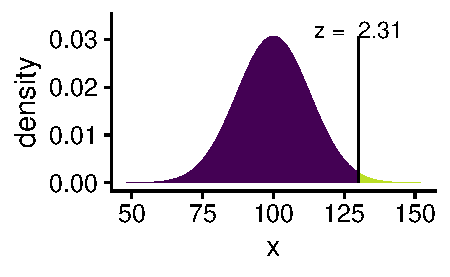
\includegraphics[width=0.6\linewidth]{figure/probs3-1} 

}


\begin{kframe}\begin{verbatim}
## [1] 0.9894919
\end{verbatim}
\end{kframe}
\end{knitrout}
	
	\pause 
	
	\begin{itemize}
		\item \texttt{pnorm} returns the integral from $-\infty$ to $q$ for a $\mathcal{N}(\mu, \sigma)$
		\item \texttt{pnorm} goes from \textit{quantiles} (think $Z$ scores) to probabilities
	\end{itemize}
	
\end{frame}



\begin{frame}[fragile]{For quantiles we use $qnorm$}
	
	
	
\begin{knitrout}\tiny
\definecolor{shadecolor}{rgb}{0.969, 0.969, 0.969}\color{fgcolor}\begin{kframe}
\begin{alltt}
\hlstd{stats}\hlopt{::}\hlkwd{qnorm}\hlstd{(}\hlkwc{p} \hlstd{=} \hlnum{0.0104}\hlstd{,} \hlkwc{mean} \hlstd{=} \hlnum{100}\hlstd{,} \hlkwc{sd} \hlstd{=} \hlnum{13}\hlstd{)}
\end{alltt}
\begin{verbatim}
## [1] 69.94926
\end{verbatim}
\end{kframe}
\end{knitrout}
	
	\pause 
	
\begin{knitrout}\tiny
\definecolor{shadecolor}{rgb}{0.969, 0.969, 0.969}\color{fgcolor}\begin{kframe}
\begin{alltt}
\hlstd{mosaic}\hlopt{::}\hlkwd{xqnorm}\hlstd{(}\hlkwc{p} \hlstd{=} \hlnum{0.0104}\hlstd{,} \hlkwc{mean} \hlstd{=} \hlnum{100}\hlstd{,} \hlkwc{sd} \hlstd{=} \hlnum{13}\hlstd{)}
\end{alltt}
\end{kframe}

{\centering 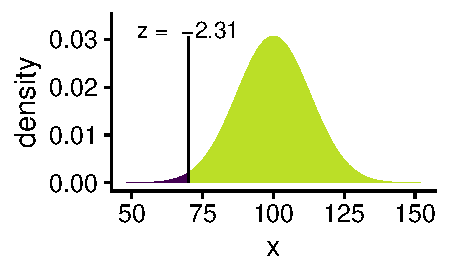
\includegraphics[width=0.6\linewidth]{figure/probs5-1} 

}


\begin{kframe}\begin{verbatim}
## [1] 69.94926
\end{verbatim}
\end{kframe}
\end{knitrout}
	
	\pause 
	
	\small{
		\begin{itemize}
			\item \texttt{qnorm} answers the question: What is the Z-score of the $p$th percentile of the normal distribution?
			
			\item \texttt{qnorm} goes from \textit{probabilities} to quantiles 
		\end{itemize}
	}
\end{frame}


\frame{\frametitle{The Normal distribution}
	\textcolor{blue}{Q2:} What is the probability of seeing an IQ
	score \textbf{as extreme as} (think highly unusual)  130? \\
	\begin{enumerate}
		\item Again, we find that $X=130$ is the same percentile of the
		IQ Normal distribution as $Z=2.31$ is of the standard Normal. \pause
		\item To see what scores are as extreme, we want to know the
		probability that $Z>$2.31 or that $Z<$-2.31. \pause
		\item As we saw previously, $P(Z > 2.31) = P(Z < -2.31) =
		0.0104$, so the probability of seeing an IQ as extreme or more
		so than 130 is $2\times0.0104 = 0.0208$.
	\end{enumerate}
}


\begin{frame}[fragile]{Finding tail probabilities}
	
	
	
\begin{knitrout}\tiny
\definecolor{shadecolor}{rgb}{0.969, 0.969, 0.969}\color{fgcolor}\begin{kframe}
\begin{alltt}
\hlcom{# lower.tail = TRUE is the default}
\hlstd{stats}\hlopt{::}\hlkwd{pnorm}\hlstd{(}\hlkwc{q} \hlstd{=} \hlopt{-}\hlnum{2.31}\hlstd{,} \hlkwc{mean} \hlstd{=} \hlnum{0}\hlstd{,} \hlkwc{sd} \hlstd{=} \hlnum{1}\hlstd{,} \hlkwc{lower.tail} \hlstd{=} \hlnum{TRUE}\hlstd{)} \hlopt{+}
\hlstd{stats}\hlopt{::}\hlkwd{pnorm}\hlstd{(}\hlkwc{q} \hlstd{=} \hlnum{2.31}\hlstd{,} \hlkwc{mean} \hlstd{=} \hlnum{0}\hlstd{,} \hlkwc{sd} \hlstd{=} \hlnum{1}\hlstd{,} \hlkwc{lower.tail} \hlstd{=} \hlnum{FALSE}\hlstd{)}
\end{alltt}
\begin{verbatim}
## [1] 0.02088815
\end{verbatim}
\end{kframe}
\end{knitrout}
	
	\pause 
	
\begin{knitrout}\tiny
\definecolor{shadecolor}{rgb}{0.969, 0.969, 0.969}\color{fgcolor}\begin{kframe}
\begin{alltt}
\hlstd{mosaic}\hlopt{::}\hlkwd{xpnorm}\hlstd{(}\hlkwc{q} \hlstd{=} \hlkwd{c}\hlstd{(}\hlopt{-}\hlnum{2.31}\hlstd{,}\hlnum{2.31}\hlstd{),} \hlkwc{mean} \hlstd{=} \hlnum{0}\hlstd{,} \hlkwc{sd} \hlstd{=} \hlnum{1}\hlstd{)}
\end{alltt}
\end{kframe}

{\centering 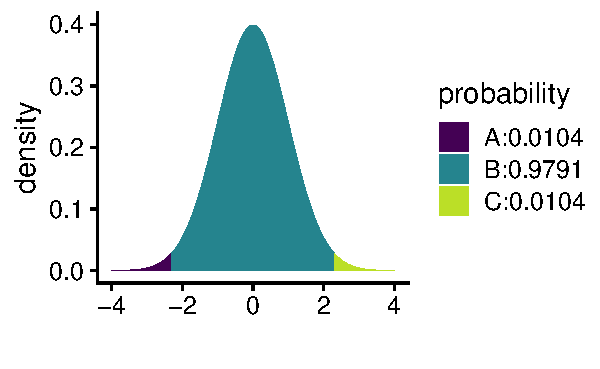
\includegraphics[width=0.6\linewidth]{figure/probs7-1} 

}


\begin{kframe}\begin{verbatim}
## [1] 0.01044408 0.98955592
\end{verbatim}
\end{kframe}
\end{knitrout}
	
	
\end{frame}



\begin{frame}[fragile]{The Normal distribution}
	\textcolor{blue}{Q3:}
	What is the 75$^{th}$ percentile of the IQ scores distribution? \\
	We now have to reverse the sequence of steps: \pause
	\begin{itemize}
		\item \textcolor{blue}{Ask yourself:} What $Z$ value corresponds to a probability of 0.75? Should you use \texttt{pnorm} or \texttt{qnorm}? \pause
		
\begin{knitrout}\tiny
\definecolor{shadecolor}{rgb}{0.969, 0.969, 0.969}\color{fgcolor}\begin{kframe}
\begin{alltt}
\hlstd{mosaic}\hlopt{::}\hlkwd{xqnorm}\hlstd{(}\hlkwc{p} \hlstd{=} \hlnum{0.75}\hlstd{,} \hlkwc{mean} \hlstd{=} \hlnum{100}\hlstd{,} \hlkwc{sd} \hlstd{=} \hlnum{13}\hlstd{)}
\end{alltt}
\end{kframe}

{\centering 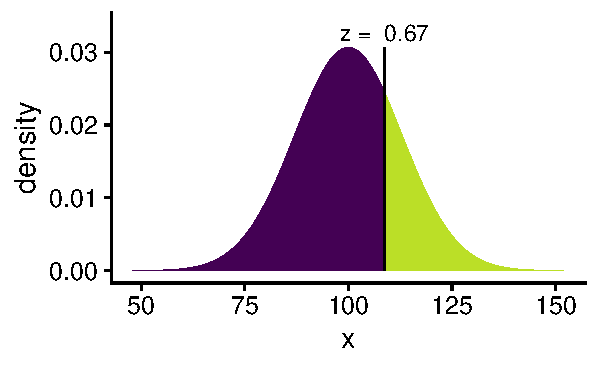
\includegraphics[width=0.6\linewidth]{figure/probs8-1} 

}


\begin{kframe}\begin{verbatim}
## [1] 108.7684
\end{verbatim}
\end{kframe}
\end{knitrout}
		
		\item[]
	\end{itemize} This tells us that 75\% of the IQ scores fall below 108.8. 
\end{frame}


\begin{frame}[fragile]{Empirical Rule or 68-95-99.7\% Rule}
	
	In any normal distribution with mean $\mu$ and standard deviation $\sigma^2$:
	\begin{itemize}
		\setlength\itemsep{2em}
		\item Approximately 68\% of the data fall within one standard deviation of the mean.
		\item Approximately 95\% of the data fall within two standard deviations of the mean.
		\item Approximately 99.7\% of the data fall within three standard deviations of the mean.
	\end{itemize}
\end{frame}



\begin{frame}[fragile]{Empirical Rule or 68-95-99.7\% Rule}
	
	\framedgraphic{6899rule.png}
	
\end{frame}

\frame{\frametitle{Properties of Normal random variables} Special
	properties of the Normal distribution:
	\begin{itemize}
		\item[] \item In $Y$ is a Normal random variable, then so is $a+bY$. \pause
		\item[] \item If $X$ and $Y$ are two Normal random variables, then
		$X+Y$ is a Normal random variable. What is the mean and variance of this new random
		variable? \pause
		\item[] \item If $X$ and $Y$ are two Normal random variables and
		$\rho_{XY}=0$ (correlation between $X$ and $Y$), then $X$ and $Y$ are independent.
	\end{itemize}
} \frame{\frametitle{Properties of Normal random variables} 
	Let $Y_1,...,Y_n \sim \mathcal{N}(\mu,\sigma)$, and let each $Y_i$
	be independent of the others. (\textcolor{blue}{think simple random sample})\\ \ \\
	
	Then $\overline{Y} = \frac{1}{n}\sum_{i=1}^n Y_i$ has what distribution? \pause
	\begin{itemize}
		\item The sum of Normal random variables is Normal, so $\overline{Y}$ is a
		Normal random variable. \pause
		\item $E(\overline{Y}) = \frac{1}{n}\sum_{i=1}^n E(Y_i) =  \frac{1}{n}\sum_{i=1}^n \mu =
		\mu$.\pause
		\item $Var(\overline{Y}) = Var(\frac{1}{n}\sum_{i=1}^n Y_i) =  \frac{1}{n^2}\sum_{i=1}^n Var(Y_i) =
		\sigma^2/n$. \pause 
		\item Standard Error of $\overline{Y}$ = $\sqrt{Var(\overline{Y})} = \sigma / \sqrt{n}$
	\end{itemize}
}



\begin{comment}
\frame{\frametitle{Properties of estimators} As we have discussed,
there are several properties that we want in an estimator:
\begin{enumerate}
\item Unbiased: the expected value (mean) of the estimator is equal to the
parameter
\begin{itemize}
\item The sample mean, $\overline{x}$, is unbiased for the population
mean, $\mu$
\end{itemize} \pause
\item Consistent: as sample size gets larger, the estimator gets
closer to the parameter \pause
\end{enumerate}
How do we go about finding an estimator might have good properties?
\\ \ \\ \pause

One approach to finding good estimates is to ask ``What value of the parameter is most
likely, given the data that I observed?'' Such an estimate is a \textbf{Maximum
Likelihood Estimator} (MLE). } \frame{\frametitle{Maximum Likelihood Estimators} Suppose
we have a sample $x_1,x_2,...,x_n$ from a Normally distributed population with unknown
mean $\mu$ and known variance $\sigma^2=1$. We want to estimate $\mu$ from the data. The
obvious estimator is the sample mean, $\bar{x}$. \\ \ \\\pause

We have already shown that the sample mean is unbiased (that is,
$E[\bar{x}] = \mu$) and that we can control its variability through
the size of our sample (since Var$[\bar{x}] = \sigma^2/n$). Are
there other theoretically justifications for using the sample mean?
} \frame{\frametitle{Maximum Likelihood Estimators} It turns out
that $\bar{x}$ maximizes the probability of the observed data, given
$\mu$. An estimator that has this property is a \textbf{maximum
likelihood estimator}.
\begin{figure}
\begin{center}
\epsfig{figure=MLE-R-1.eps,width=3in,height=2.7in}
\end{center}
\end{figure}
} \frame{\frametitle{Maximum Likelihood Estimators} It turns out
that $\bar{x}$ maximizes the probability of the observed data, given
$\mu$. An estimator that has this property is a \textbf{maximum
likelihood estimator}.
\begin{figure}
\begin{center}
\epsfig{figure=MLE-R-2.eps,width=3in,height=2.7in}
\end{center}
\end{figure}
} \frame{\frametitle{Maximum Likelihood Estimators} It turns out
that $\bar{x}$ maximizes the probability of the observed data, given
$\mu$. An estimator that has this property is a \textbf{maximum
likelihood estimator}.
\begin{figure}
\begin{center}
\epsfig{figure=MLE-R-3.eps,width=3in,height=2.7in}
\end{center}
\end{figure}
} \frame{\frametitle{Maximum Likelihood Estimators} It turns out
that $\bar{x}$ maximizes the probability of the observed data, given
$\mu$. An estimator that has this property is a \textbf{maximum
likelihood estimator}.
\begin{figure}
\begin{center}
\epsfig{figure=MLE-R-4.eps,width=3in,height=2.7in}
\end{center}
\end{figure}
}
content...
\end{comment}

\begin{comment}
\frame{\frametitle{Maximum Likelihood Estimators} For each data
point, the probability density function is given by:
\[ f(x_i|\mu,\sigma) = \frac{1}{\sqrt{2p}\sigma}\exp\left(-\frac{(x_i-\mu)^2}{2\sigma^2}\right). \]
Since the data are independent, we can use the product rule:
\begin{eqnarray*}
f(x_1,x_2,...,x_n|\mu,\sigma) & = &
\prod_{i=1}^n\frac{1}{\sqrt{2p}\sigma}\exp\left(-\frac{(x_i-\mu)^2}{2\sigma^2}\right)\\
& = & \frac{1}{\sqrt{2p}\sigma}\exp\left(-\frac{\sum_{i=1}^n(x_i-\mu)^2}{2\sigma^2}\right).\\
\end{eqnarray*}
This function is called a \textbf{likelihood function}; it describes
the likelihood (or the probability) of the observed data for a given
value of $\mu$ (and $\sigma$). }

\frame{\frametitle{Maximum Likelihood Estimators} We want to maximize this probability
function. That is, we want to find the value of $\mu$ that gives the highest probability
to the data we observed. \\ \ \\ \pause

From calculus, we know that we maximize a function by taking its derivative and set it
equal to zero. Doing this and simplifying gives
\[\frac{1}{2\sigma^2}\sum_{i=1}^n2(x_i-\mu) = 0.\] \pause

This implies \[\sum_{i=1}^n(x_i-\mu) = \sum_{i=1}^nx_i - n\mu  = 0\]
so that the likelihood is maximized at $\mu=
\frac{1}{n}\sum_{i=1}^nx_i = \bar{x}.$ Thus the MLE of $\mu$ is
$\bar{x}.$ }
\end{comment}

%%%%%%%%%%%%%%%%%%%%%%%%%%%%%%%%%%%%%%%%%%%%%%%%%%%%%%%%%%%%%%%%%%%
\begin{comment}
\subsection{Normal approximation to binomial}

\frame{\frametitle{Normal approximation of the binomial
distribution} Suppose we take a large random sample of size $n$
in our population, and count $X$, the number of `successes'
(success could be the event of having MS, the event of
exercising more than twice per week, etc.).
\begin{itemize}
\item We can view $X$ as being sampled from a Binomial$(n,p)$
distribution... \pause
\item OR we can view $X$ as the sum of $n$ binary variable
$Y_1$,...,$Y_n$ where $Y_i \sim$ Binomial$(1,p)$.
\item The Binomial$(1,p)$ distribution is also called a
Bernoulli$(p)$ distribution.
\end{itemize}
} \frame{\frametitle{Normal approximation of the binomial} Now
$\hat{p} = X/n$ is the sample proportion of successes, which is an
estimate of $p$, the mean of the Bernoulli$(p)$ distribution. \\ \ \\

If $\min(np,n(1-p)) \ge 10$, then we have
\begin{itemize}
\item $X$ is approximately distributed $\mathcal{N}(np,\sqrt{np(1-p)})$
\item $\hat{p}$ is approximately distributed $\mathcal{N}(\quad,\quad\quad)$
\end{itemize}
} \frame{\frametitle{Normal approximation of the binomial}
Why is this true? \\
\begin{itemize}
\item[] \item For $\hat{p}$, this is easy to explain: $\hat{p}$ is just a
sample average of Bernoulli random variables, since \[\hat{p} = X/n =
(\frac{1}{n}\sum_{i=1}^n Y_i),\] and so the CLT applies. \pause
\item[] \item But what about $X$? $X$ is just a linear
transformation of $\hat{p}$, since $X = n\hat{p}$, and linear
combinations of (approximately) Normal random variables are
(approximately) Normal.
\item[] \item The approximation is best when $p$ is near 0.5 (which makes the
distribution of $X$ symmetric) and/or $n$ is large.
\end{itemize}
} \frame{\frametitle{Normal approximation of the binomial}
\begin{figure}
\begin{center}
\epsfig{figure=NormalApproxBino.eps,width=3.3in,height=3.3in}
\end{center}
\end{figure}
}

\frame{\frametitle{Normal approximation of the binomial}
Suppose we collect a simple random sample of $n=150$ health
care workers in India. What is the probability that $X=80$ or
more of the individuals show antibody response to TB
(indicating previous TB exposure) if $p=0.6$? \\ \ \\

Our binomial tables do not cover the cases for $n$ as large as
150. Also, calculating
\[ P(X = 80\hbox{ out of } 150) =
\frac{150!}{(150-80)!80!}0.6^{80}0.4^{(150-80)}\] is difficult at
best. 150! is a number that is over 250 digits long, and $0.6^{80}$
is very, very small. Not only that, but to find $P(X \ge 80\hbox{ out of } 150)$, we would have to sum 70
terms to calculate this probability. }

\frame{\frametitle{Normal approximation of the binomial} Let's
use the Normal approximation!! \\ \ \\
First, we need to calculate the mean and variance of the
distribution:
\begin{eqnarray*}
\mu & = & np = 150\times0.6 = 90\\
\sigma^2 & = & np(1-p) = 150\times0.6\times0.4 = 36
\end{eqnarray*} \pause
The Normal approximation to the binomial is improved by using a
\textbf{continuity correction}, so that instead of estimation $P(X
\ge 80|X\sim\hbox{Bino}(150,0.6))$ we estimate $P(X \ge
79.5|X\sim\hbox{Bino}(150,0.6))$, and approximate this by $P(X \ge
79.5|X\sim\mathcal{N}(90,6))$. }

\frame{\frametitle{Normal approximation of the binomial}
{\small
\[P(X \ge 80|X\sim\hbox{Bino}(150,0.6)) = P(X \ge
79.5|X\sim\hbox{Bino}(150,0.6))\]
\begin{eqnarray*}
\qquad \qquad & \approx & P(X \ge 79.5|X\sim\mathcal{N}(90,6))\\
\pause
& = & P\left(\frac{X-\mu}{\sigma} \ge
\frac{79.5-\mu}{\sigma}|X\sim\mathcal{N}(90,6)\right)\\ \pause
& = & P\left(\frac{X-90}{6} \ge
\frac{79.5-90}{6}|X\sim\mathcal{N}(90,6)\right)\\ \pause
& = & P\left(Z \ge -1.75|Z\sim\mathcal{N}(0,1)\right)\\
& = & 0.9599
\end{eqnarray*} }
}

\frame{\frametitle{Normal approximation of the binomial} What
difference does the continuity correction make? \\ \ \\ {\small
\[P(X \ge 80|X\sim\hbox{Bino}(150,0.6)) \qquad \qquad \qquad \qquad \qquad \qquad \]
\begin{eqnarray*}
\qquad \qquad & \approx & P\left(\frac{X-\mu}{\sigma} \ge
\frac{80-\mu}{\sigma}|X\sim\mathcal{N}(90,6)\right)\\
& = & P\left(\frac{X-90}{6} \ge
\frac{80-90}{6}|X\sim\mathcal{N}(90,6)\right)\\
& = & P\left(Z \ge -1.667|Z\sim\mathcal{N}(0,1)\right)\\
& = & 0.9522
\end{eqnarray*} }
...In this case, it doesn't matter much. BUT...
}

\frame{\frametitle{Normal approximation of the binomial} Now we
ask the question, ``What is the probability that exactly $X=80$
of the health care workers show antibody response to TB?'' \\ \ \\

If we \textit{don't} use the continuity correction, we find:
{\small
\[P(X = 80|X\sim\hbox{Bino}(150,0.6)) \qquad \qquad \qquad \qquad \qquad \qquad \]
\begin{eqnarray*}
\qquad \qquad & \approx & P\left(\frac{X-\mu}{\sigma} = \frac{80-\mu}{\sigma}|X\sim\mathcal{N}(90,6)\right)\\
& = & P\left(\frac{X-90}{6} = \frac{80-90}{6}|X\sim\mathcal{N}(90,6)\right)\\
& = & P\left(Z= -1.667|Z\sim\mathcal{N}(0,1)\right)\\
& = & 0
\end{eqnarray*}  }
(Why this this probability zero?)
}

\frame{\frametitle{Normal approximation of the binomial} Using
the continuity correction gives {\small
\[P(X = 80|X\sim\hbox{Bino}(150,0.6)) \qquad \qquad \qquad \qquad \qquad \qquad \]
\begin{eqnarray*}
\qquad \qquad & = & P(79.5 \le X \le
80.5|X\sim\hbox{Bino}(150,0.6))\\
& \approx & P(79.5 \le X \le 80.5|X\sim\mathcal{N}(90,6))\\
& = & P\left(\frac{79.5-\mu}{\sigma} \le \frac{X-\mu}{\sigma} \le
\frac{80.5-\mu}{\sigma}|X\sim\mathcal{N}(90,6)\right)\\
& = & P\left(\frac{79.5-90}{6}| \le \frac{X-90}{6} \le
\frac{80.5-90}{6}|X\sim\mathcal{N}(90,6)\right)\\
& = & P\left(-1.75 < Z \le -1.583|Z\sim\mathcal{N}(0,1)\right)\\
& = & 0.0166
\end{eqnarray*}} \pause

Using the binomial distribution formula, the exact answer is
0.01659816. The Normal approximation with the continuity
correction is correct to 4 decimal places.}
\end{comment}


	
\begin{frame}[fragile]{Session Info}
	\tiny
	
\begin{knitrout}\tiny
\definecolor{shadecolor}{rgb}{0.969, 0.969, 0.969}\color{fgcolor}\begin{kframe}
\begin{verbatim}
R version 4.0.4 (2021-02-15)
Platform: x86_64-pc-linux-gnu (64-bit)
Running under: Pop!_OS 21.04

Matrix products: default
BLAS:   /usr/lib/x86_64-linux-gnu/openblas-pthread/libblas.so.3
LAPACK: /usr/lib/x86_64-linux-gnu/openblas-pthread/libopenblasp-r0.3.13.so

attached base packages:
[1] tools     stats     graphics  grDevices utils     datasets  methods  
[8] base     

other attached packages:
 [1] DT_0.16           mosaic_1.7.0      Matrix_1.3-2      mosaicData_0.20.1
 [5] ggformula_0.9.4   ggstance_0.3.4    lattice_0.20-41   kableExtra_1.2.1 
 [9] socviz_1.2        gapminder_0.3.0   here_0.1          NCStats_0.4.7    
[13] FSA_0.8.30        forcats_0.5.1     stringr_1.4.0     dplyr_1.0.7      
[17] purrr_0.3.4       readr_1.4.0       tidyr_1.1.3       tibble_3.1.3     
[21] ggplot2_3.3.5     tidyverse_1.3.0   knitr_1.33       

loaded via a namespace (and not attached):
 [1] fs_1.5.0           lubridate_1.7.9    webshot_0.5.2      httr_1.4.2        
 [5] rprojroot_2.0.2    backports_1.2.1    utf8_1.2.2         R6_2.5.1          
 [9] DBI_1.1.1          colorspace_2.0-2   withr_2.4.2        tidyselect_1.1.1  
[13] gridExtra_2.3      leaflet_2.0.3      curl_4.3.2         compiler_4.0.4    
[17] cli_3.0.1          rvest_1.0.0        pacman_0.5.1       xml2_1.3.2        
[21] ggdendro_0.1.22    labeling_0.4.2     mosaicCore_0.8.0   scales_1.1.1      
[25] digest_0.6.27      foreign_0.8-81     rmarkdown_2.9.7    rio_0.5.16        
[29] pkgconfig_2.0.3    htmltools_0.5.2    highr_0.9          dbplyr_1.4.4      
[33] fastmap_1.1.0      htmlwidgets_1.5.3  rlang_0.4.11       readxl_1.3.1      
[37] rstudioapi_0.13    farver_2.1.0       generics_0.1.0     jsonlite_1.7.2    
[41] crosstalk_1.1.1    zip_2.2.0          car_3.0-9          magrittr_2.0.1    
[45] Rcpp_1.0.7         munsell_0.5.0      fansi_0.5.0        abind_1.4-5       
[49] lifecycle_1.0.0    stringi_1.7.3      carData_3.0-4      MASS_7.3-53.1     
[53] plyr_1.8.6         grid_4.0.4         blob_1.2.1         ggrepel_0.8.2     
[57] crayon_1.4.1       cowplot_1.1.0      haven_2.3.1        splines_4.0.4     
[61] hms_1.0.0          pillar_1.6.2       reprex_0.3.0       glue_1.4.2        
[65] evaluate_0.14      data.table_1.14.0  modelr_0.1.8       vctrs_0.3.8       
[69] tweenr_1.0.1       cellranger_1.1.0   gtable_0.3.0       polyclip_1.10-0   
[73] assertthat_0.2.1   TeachingDemos_2.12 xfun_0.25          ggforce_0.3.2     
[77] openxlsx_4.1.5     broom_0.7.2        viridisLite_0.4.0  ellipsis_0.3.2    
\end{verbatim}
\end{kframe}
\end{knitrout}
	
\end{frame}



\end{document}







